%无限深势阱中解定态薛定谔方程

\pentry{定态薛定谔方程%引用未完成
,二阶常系数齐次微分方程%引用未完成
}

只考察质量为 $m$ 的粒子沿 $x$ 方向的运动情况.% 有没有地方可以说明一下矢量空间, 我们只在 x 空间解决问题
势能函数为
\begin{equation}
V(x) = \leftgroup{
&0 \quad &&(0 \les x \les a)\\
+&\infty  &&(x < 0 \ \text{或}\  x > a)
}\end{equation}

\begin{figure}[ht]
\centering
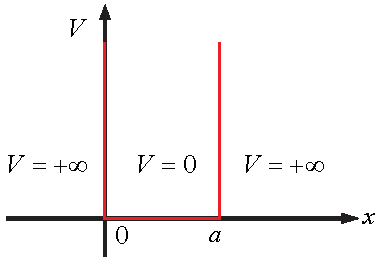
\includegraphics[width=6cm]{./figures/ISW.pdf}
\caption{无限深势阱} \label{ISW_fig1}
\end{figure}
求解定态薛定谔方程 % 链接未完成
\begin{equation}
-\frac{\hbar ^2}{2m} \dv[2]{x} \psi(x) + V(x) = E\psi(x)
\end{equation} 
\subsection{结论} 

第 $n$ 个能级为
\begin{equation}
E_n = \frac{\pi^2 \hbar^2}{2m a^2} n^2 \quad (n = 1,2,3...)
\end{equation}
能量的本征波函数为
\begin{equation}
\psi(x) = \sqrt{\frac{2}{a}} \sin(\frac{n\pi }{a} x)
\end{equation}

\subsection{推导} 
先考虑势阱内部($0 \les x \les a$, $V = 0$),方程变为
\begin{equation}
-\frac{\hbar^2}{2m} \dv[2]{x} \psi(x) = E\psi(x) 
\end{equation}
这是二阶常系数齐次微分方程.通解为
\begin{equation}
\psi(x) = C_1\cos(kx) + C_2 \sin(kx) \qquad
k = \frac{\sqrt{2mE}}{\hbar}
\end{equation} 
其中

(通解也可以写成指数函数 $C\E^{\I kx}$, 加上边界条件后的结论一样)
现在讨论边界条件: 在有限深势阱束缚态中将会看到,如果势阱外部势能是有限值,波函数将会按照指数函数衰减,势能越高衰减得越快.而现在势阱外部势能为无穷大,就可以直接认为波函数在势阱外部始终为零.所以边界条件为
\begin{equation}
\psi(0) = 0, \quad \psi(a) = 0
\end{equation}
这两个条件代入以上通解中,解得
\begin{equation}
C_2 = 0, \quad k = \frac{n\pi}{a}  \ \ (n = 1,2,3\dots)
\end{equation}

$C_1$ 的取值暂时不能确定,但先将通解写为 $\psi(x) = C\sin(\frac{n\pi }{a}x)$, 常数 $C$ 就可以通过波函数的归一化%(链接未完成)
来确定:
\begin{equation}
1 = \int_{-\infty }^{+\infty } \abs{\psi(x)}^2 \dd{x}  = \int_{-a}^{+a} \abs{C\sin(\frac{n\pi }{a} x)}^2 \dd{x}  = \abs{C}^2 \frac{a}{2}
\end{equation}
严格来说, $C$ 可以是复数,解为 $C = \sqrt{2/a} \E^{\I\theta}$. 但是为了方便通常把归一化常数中的相位因子$\E^{\I\theta}$ 默认为 $1$. 所以归一化的波函数为
\begin{equation}
\psi(x) = \sqrt{\frac{2}{a}} \sin(\frac{n\pi }{a}x)
\end{equation}
另外,由
\begin{equation}
\frac{\sqrt{2mE}}{\hbar} = k = \frac{n\pi }{a}
\end{equation}
可以得出能级是离散的结论.即
\begin{equation}
E_n = \frac{\pi^2\hbar^2}{2m a^2} n^2 \quad (n = 1,2,3\dots)
\end{equation}

